% Chapter 1

\chapter{Evaluation} % Main chapter title

\label{chap_eval} % For referencing the chapter elsewhere, use \ref{Chapter1}

%----------------------------------------------------------------------------------------
This chapter contains a detailed breakdown of all the results that have been gathered during the course of this project,
with each section featuring a comparison of one distinct aspect that was tested for. All of these results and comparisons are to be taken with a large grain of salt however, as due to time and resource constraints all of these tests were done with somewhat suboptimal hyperparameter configurations.
Using more optimized or simply different parameter configurations might yield vastly different results.
\section{Method of Recording and Evaluating}
Most of the logs utilized for this evaluation both of the OpenAI Baselines algorithms and the A3C algorithm were recorded using the \lstinline{bench.monitor} module supplied with the OpenAI Baselines Repository. Nevertheless, for some scenarios there are only legacy plots available for the A3C algorithm, that were made before the baselines scripts were integrated in this project and that could not be rerecorded in time for this thesis.\\ The monitor module has multiple different output formats, of which the JsonOutput was used. The monitor, acting as an additional wrapper around the environment wrappers that are already in place, records their results independently in separate log files. Each line in the json output log files, represents the result of one episode, with the exception of the first line, which contains general environment information. Recorded for each episode are the total cumulative reward at the end of the episode, the length of the episode given by the number of steps the algorithm took, and the time in seconds, since the beginning of the test run. These values are then plotted using the \lstinline{plot_baselines} module as described in section \ref{sec:plotbase}.

In general the tests were comparatively short, with initial test runs being 80 million steps long in total which was increased to 120 million for the more difficult scenarios. Only 3 tests were run, that were longer than that, all of these in cases were no adequate result was achieved during multiple runs of 120 million steps. In comparison, DeepMind's tests that were shown in the introductory paper form PySC2 ran for 600 million steps each. Although tests were done for almost every scenario with each of the 3 algorithms, in order to compare them in section \ref{sec:eval_algo}, most other sections in this chapter feature results exclusively from the ACKTR algorithm. This is again due to resource constraints and also due to the fact, that ACKTR was thought of as the best of the three.  


\section{Scenarios}
This section will compare the different scenarios and in particular how challenging they were to solve. For a fair comparison of all scenarios they are compared using the scores garnered by training with action arguments enabled, as not all scenarios have a simplified variant. The comparison between simplified variants and action argument variants will be made in section \ref{sec:eval_aa}. Also, not the results of all algorithms are depicted in this section, and instead only the best and/or most interesting results for each scenario are discussed here. Furthermore, the Network architectures and most of the parameters like for example the number of parallel environments remained the same between all tests. The only parameter modified in this comparison is the learning rate. The reward graphs shown contain the rewards from the training with the learning rate with which the algorithm was able to obtain the best rewards. 

\subsection{Find Ultralisk}
The Find Ultralisk Scenario was expected to be the easiest scenario of all, and largely this expectation was fulfilled. All of the tested algorithms had little trouble obtaining close to the maximum rewards possible somewhat consistently. Additionally they were able to learn it with a very steep reward ascend due to a high learning rate, an example of which is shown in Figure \ref{fig:fu_rew}. This example also shows a clear difference between the progression of the maxmimum of all environments and the mean. While the smoothed maximum stagnates after the first steep ascend, the mean is still increasing even at the end of the training session, as the network gets more and more consistent. 

\begin{figure}[htb]
  \centering
      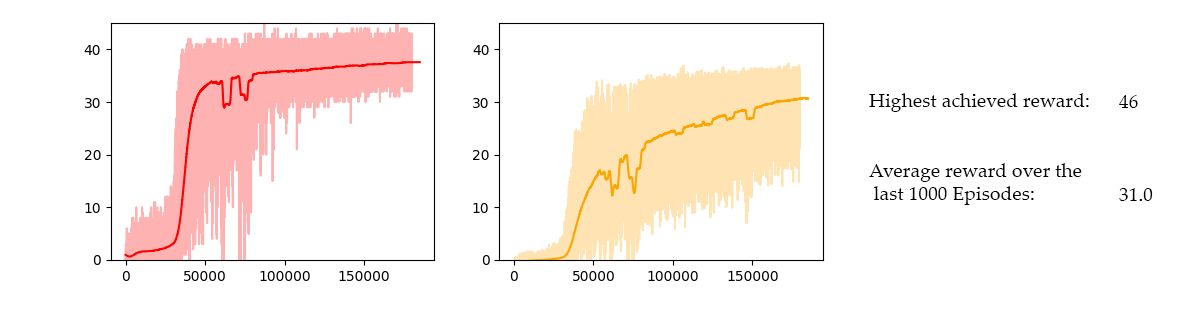
\includegraphics[width=1\textwidth]{Figures/plots/plot_fu_acktr_coord.png}
  \caption{Reward per Episode for the Find Ultralisk Scenario with maximum over all environments(left) and mean over all environments(right)}
  \label{fig:fu_rew}
\end{figure}




\subsection{Find Ultralisk With Creep}
This scenario was considerably more difficult and also more complex with an observation space that was twice as big, which reflects in the reward graphs. Not only did this scenario take longer to learn in general, even after learning the correct strategy the policies learned were somewhat less consistent. This is likely due to the large randomness involved in the observation space as there are many different possibilities for the random placement of the creep patches. 

One interesting detail to note is that looking at the plots of the episode length and comparing them to the reward plot \ref{fig:elength} one can see, that the episode lengths progress much faster and earlier to their maximum value of 240 steps than the rewards. 

\begin{figure}[htb]
  \centering
      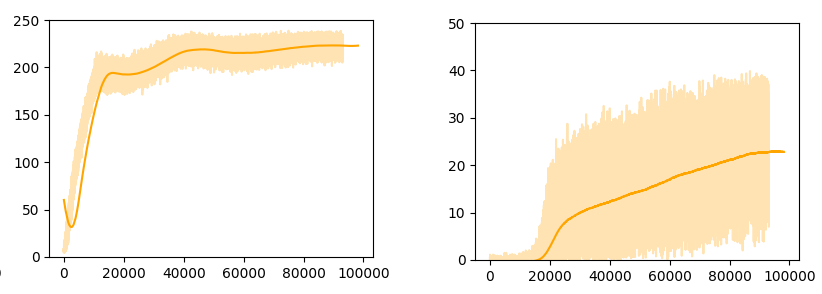
\includegraphics[width=0.8\textwidth]{Figures/plots/fuwc_elength.png}
  \caption{Comparison of Episode length/Episode (left) and Reward/Episode (right) in the Find Ultralisk with Creep Scenario. While the amount of rewards that can be obtained directly correlate to the length of the episode, the length of episode increases much earlier than the rewards after an initial dip.}
  \label{fig:elength}
\end{figure}

Evidently, the algorithm learned very quickly, that it is vital to stay alive and thus stay away from the creep, to get any more rewards at all. Actually getting more rewards by reaching the Ultralisk then only became a secondary objective, that took a while longer to achieve. This is also demonstrated in the decision making of the algorithm during an episode. If for example the algorithm controlled unit has to pass in between two patches of creep that are very close together in order to get to the Ultralisk, the algorithms tends to go back and forth for sometimes 10 to 20 steps in front of and inside of the gap, just to make sure not to touch the creep. After shuffling around for a bit it then heads straight for the Ultralisk. This decision making is even more apparent in the simplified version of this scenario, where the algorithm only has limited movement options. Figure \ref{fig:fu_shuffle} showcases this behaviour in a short sequence of steps that demonstrate part of the back and forth movement of the unit.

\begin{figure}[htb]
  \centering
      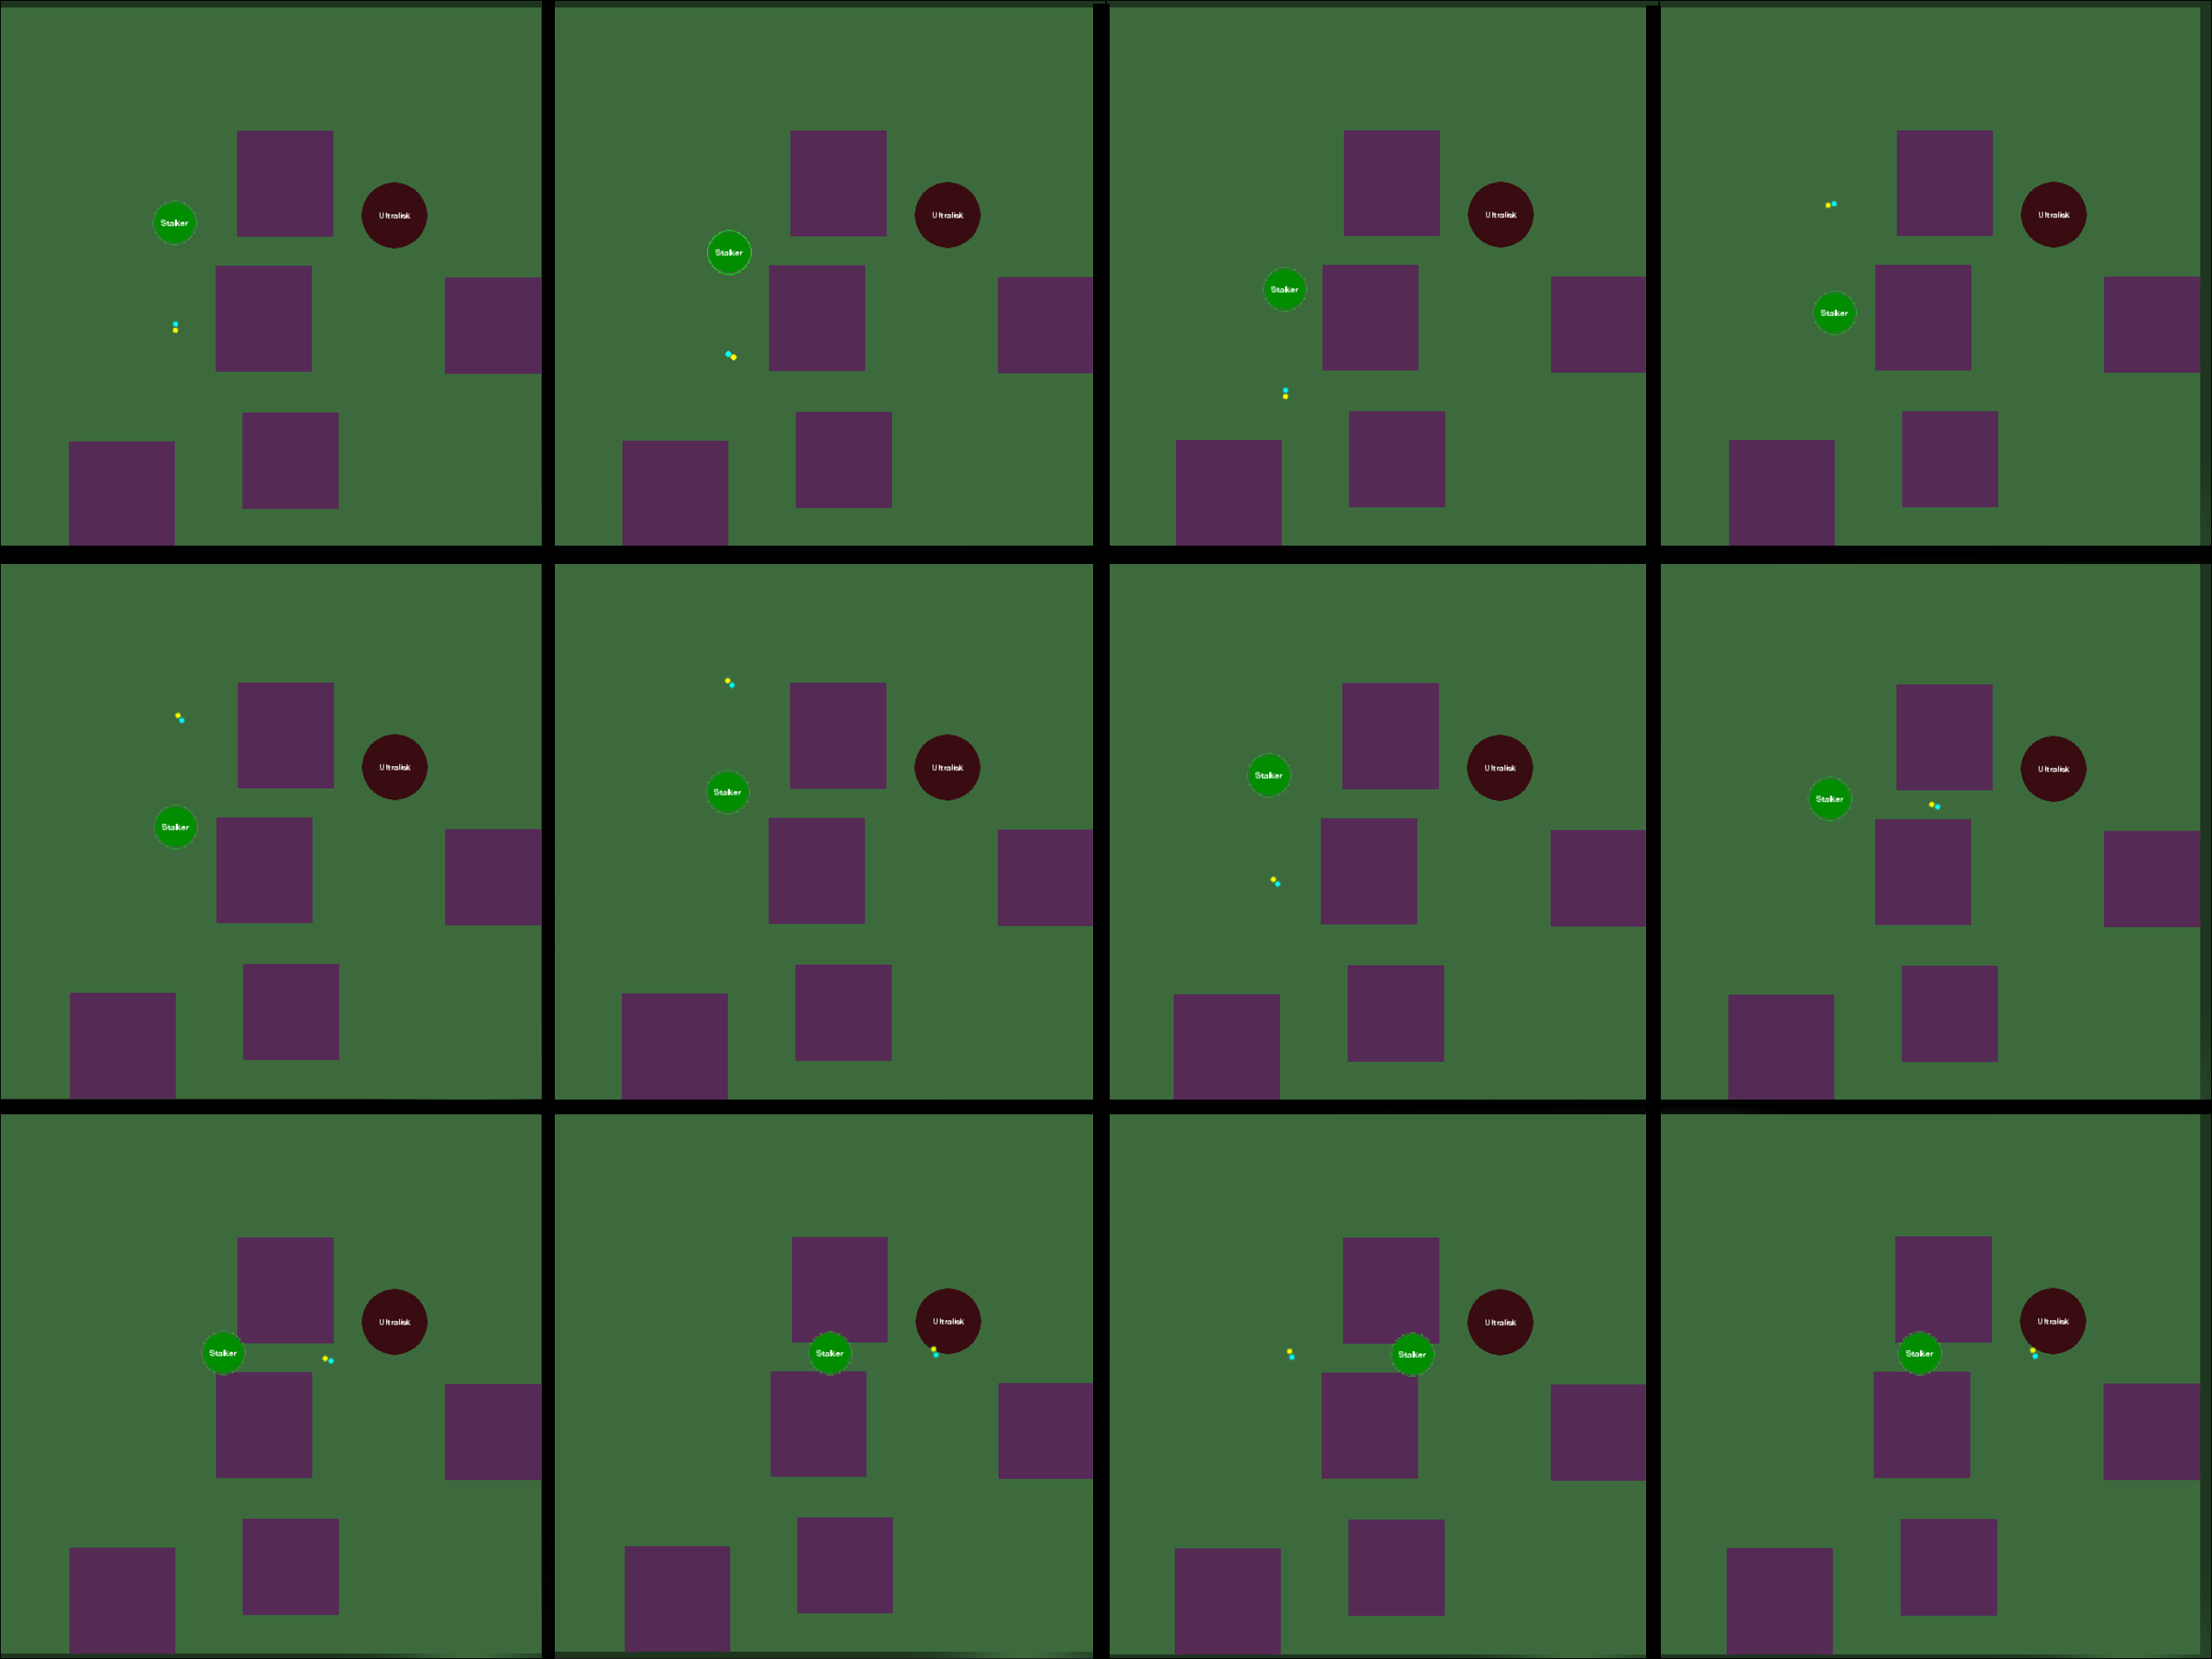
\includegraphics[width=0.8\textwidth]{Figures/fu_sequence.png}
  \caption{Excerpt of ACKTR Behaviour in Find Ultralisk with Creep Scenario when encountering a narrow path to the target. The unit moves back and forth multiple times both in front of and inside of the gap before proceeding to the target.}
  \label{fig:fu_shuffle}
\end{figure}


\subsection{Reaper vs Zergling}
The results of training on the Reaper vs Zergling Scenario show a particularly interesting difference between human play and AI play. All humans that tested this scenario played exactly as was expected: jumping up and down cliffs while attacking the group of enemy units in between jumps, thereby exploiting the terrain. The AI found a much easier solution to the original version of this scenario however. Due to the map being constrained to roughly the screen size there exists a small spot left of the lower ramp that the enemy units can not reach. As the enemy units are melee units, units located in this spot are effectively invincible. The solution of the AI therefore was naturally to move its units to this location as fast as possible and to not execute any further movement commands afterwards. While no human found this simple way of winning it is easy to see why this solution is much easier to learn and execute for the AI than the actual strategy that was expected of it.

\begin{figure}[htb]
  \centering
      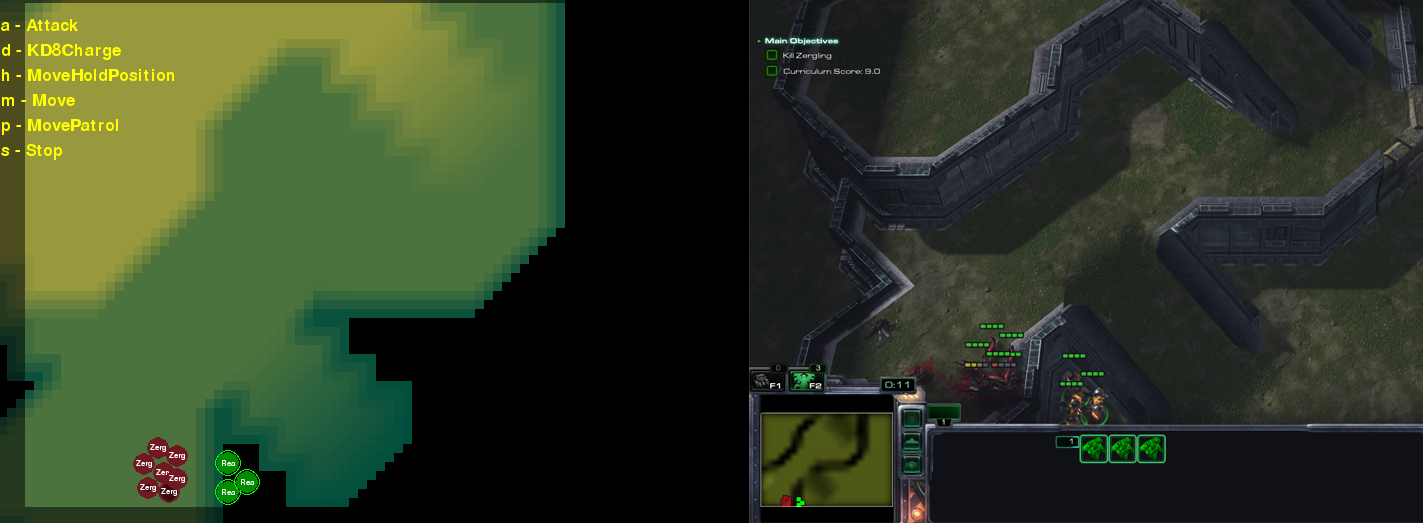
\includegraphics[width=0.8\textwidth]{Figures/rz_badramp.png}
  \caption{AI Strategy for "cheating" the original version of the Reapers vs Zergling Scenario by positioning its units in a location where they can not be reached by enemy melee units. PySC2 debug view left, real game render right.}
  \label{fig:rzstrat}
\end{figure}

In Figure \ref{fig:rzstrat} this strategy can be seen during an episode. The algorithm's units are safely tucked away in between the ramp and the cliff, and the enemy melee units can not reach them. Figure \ref{fig:rzcheat} shows the rewards obtained while learning this "cheating" strategy. While they are still far from the rewards obtained by human players, as the algorithm had problems to execute this strategy consistently, they are much better than the results for the map version that does not allow cheating displayed in Figure \ref{fig:rznocheat}. In that version only very small improvements were made over the random policy. The algorithm did not learn to exploit the terrain to it's advantage and instead simply took small steps away from the enemiy units between attacking them. While this does help a little bit, by giving the algorithm's unit slightly more time before they get defeated, eventually they are overwhelmed by the much faster enemy units. 


\begin{figure}[htb]
  \centering
      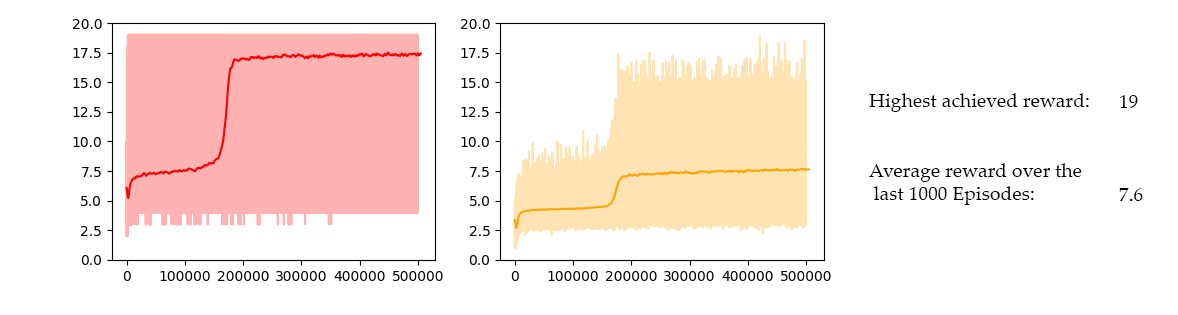
\includegraphics[width=0.8\textwidth]{Figures/plots/plot_rz_acktr_coords_cheat.png}
  \caption{Maximum and Mean Rewards for The ReaperZergling Scenario, in the version of the map that allows the algorithm to "cheat".}
  \label{fig:rzcheat}
\end{figure}

\begin{figure}[htb]
  \centering
      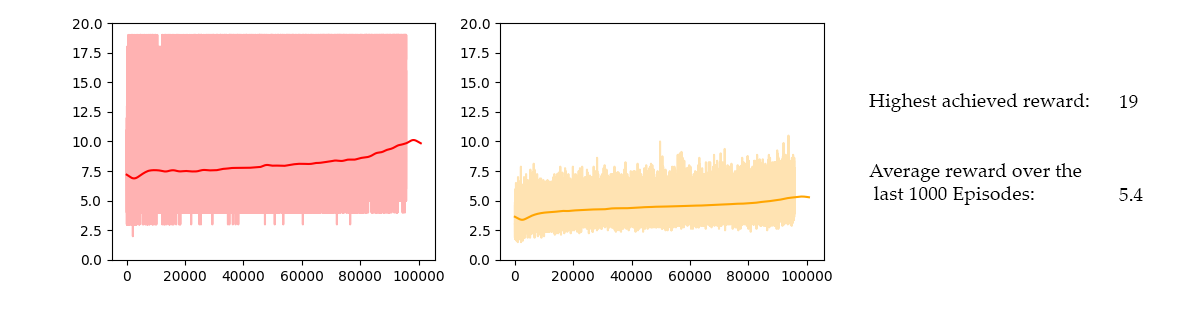
\includegraphics[width=0.8\textwidth]{Figures/plots/plot_rz_acktr.png}
  \caption{Maximum and Mean Rewards for The ReaperZergling Scenario, in the version of the map that does not allow the algorithm to "cheat".}
  \label{fig:rznocheat}
\end{figure}


\subsection{Stalkers vs Roaches}
During conception of the scenarios for this project, this scenario was considered the most difficult to learn by far. Although in comparison with the other real game scenarios of Gateway vs Zerg and Reapers vs Zergling this scenario has a slightly smaller action space and observation space it requires the most challenging strategy to be successful. In contrast to the other scenarios, where each individual action has meaningful impact on the current state in the environment, the strategy for this scenario requires a combination of actions. Namely, the select\_point Action by itself does not change much, but it is required to select wounded units in order to then teleport them to safety using the blink action. Additionally, the difficulty is increased as the requirement placed on the accuracy of screen coordinates is much higher. The Select\_Point Action needs to hit very specific units that are only 3-4 pixels high and wide in order to be effective, while in other scenarios very rough coordinates are enough to achieve close to optimal effects. 

\begin{figure}[htb]
  \centering
      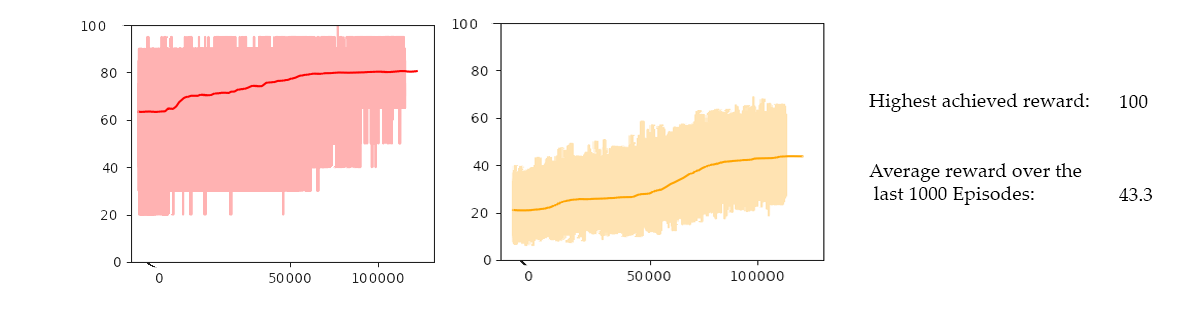
\includegraphics[width=1\textwidth]{Figures/plots/plot_sr_acktr_coord.png}
  \caption{Reward per Episode for the StalkerRoaches Scenario with maximum over all environments(left) and mean over all environments(right)}
  \label{fig:sr_rew}
\end{figure}

As Figure \ref{fig:sr_rew} shows, decent rewards were able to be obtained, in spite of these challenges. In contrast to other scenarios there is no steep reward ascend here, and instead a rather slow increase, that almost plateaus towards the end. Although average rewards are subpar compared to human results, the maximum rewards over all environments show much more promise with rewards of 100 being obtained with considerable regularity. The big discrepency between mean and maximum rewards for this scenario can be attributed to both the fact, that 32 parallel environments were used for training this scenario unlike the 8 environments used for most other scenarios and also to the generally very large inconsistency of the strategy employed by the network. 

The strategy that was learned and is demonstrated by Figure \ref{fig:srstrat} is similar to the strategy of the Reaper vs Zergling scenario in that the algorithm found a way to circumvent the problems of the scenario and instead found a considerably simpler solution. Nonetheless in this case it was not a strategy that exploits a flaw in the design of the scenario and and it is in fact a somewhat suboptimal strategy, that will never be able to achieve full rewards very consistently. What the algorithm has learned, is to effectively never use the select\_point action at all. Instead it relies solely on the blink or teleport action. As the entire army is preselected at the start of each episode, this results in the entire army getting teleported instead of, as intended, singular units. Ideally the teleport location is chosen in a a way that still puts the injured and at risk units at the back of the army, so the core concept of the strategy that was learned is the same as in the human strategy. 

\begin{figure}[htb]
  \centering
      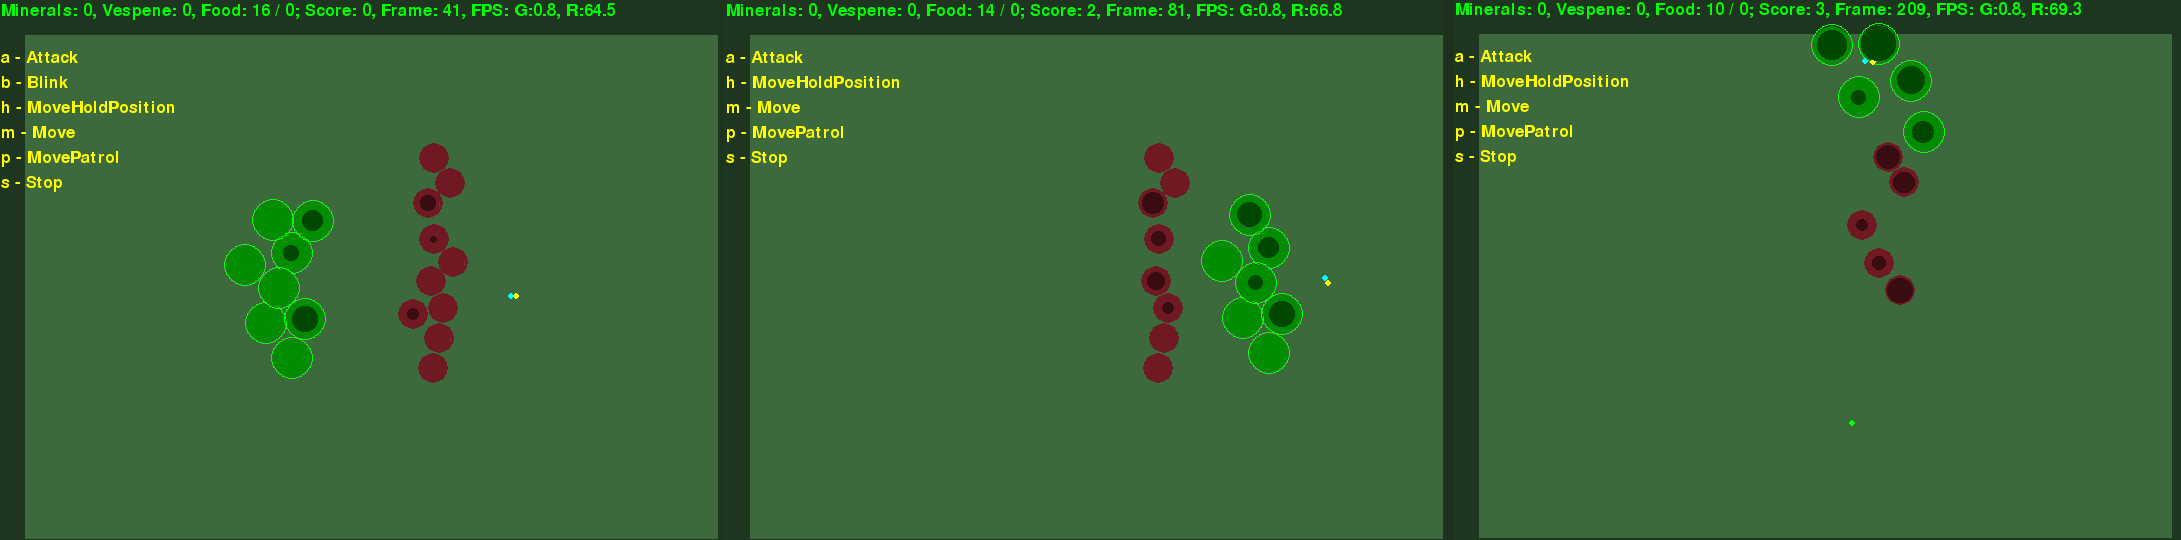
\includegraphics[width=1\textwidth]{Figures/sr_strategy.png}
  \caption{A sequence of select state snapshots demonstrating the strategy that was learned for the Stalkers vs Roaches Scenario. Instead of teleporting single units the entire army is teleported. Increasingly bigger dark green circles on a friendly unit indicate missing health.}
  \label{fig:srstrat}
\end{figure}


Teleporting the army has a few drawbacks however, that preclude it from achieving maximum rewards in most cases. The biggest one is that the blink ability has a considerable cooldown period before it can be used again, which often results in units dying while the ability is still on cooldown. Secondly, executing the blink ability causes all blinked units to stop attacking for a short duration, which makes them more vulnerable and decreases the overall damage that the army is able to inflict. Thirdly it is not always possible to teleport the entire army in a way, that injured units get placed at the back, for example if the enemy army is standing with the back ranks against a wall, effectively wasting the ability. Nonetheless, as can be seen from the reward graph the rewards were still steadily improving at the time the training was stopped. That could mean that the algorithm would not necessarily converge on this suboptimal strategy and might have been able to unlearn this strategy in order to adopt a new one given more training time.   

\subsection{Gateway vs Zerg}
This scenario is definitely the most challenging of the scenarios proposed in this project for human players. One reason for this is that in contrast to the other scenarios there is no clearly definable strategy which, if executed correctly, will always result in maximum rewards. While the general idea is to cut the enemies' army in half and force the enemy to fight your army in small groups using forcefields, this is only a very approximate goal, the path to which is constantly changing, as both armies move around the battlefield. It is also difficult, because it requires a considerable amount of foresight and prediction for, on the one hand determining were enemy routes will follow around the forcefields, and on the other hand managing the available energy of the sentry units in order to not run out of energy by placing forcefields prematurely or unnecessarily. 

The ACKTR algorithm however had little problems with this scenario and managed to gain by far the best results out of the 3 real game scenarios. It was able to not only surpass the novice StarCraft II player'S scores, but is even on par with the advanced player. Additionally surprising was, how consistent the achieved rewards were. In nearly every episode at least 90\% of the possible rewards were achieved.

\begin{figure}[htb]
  \centering
      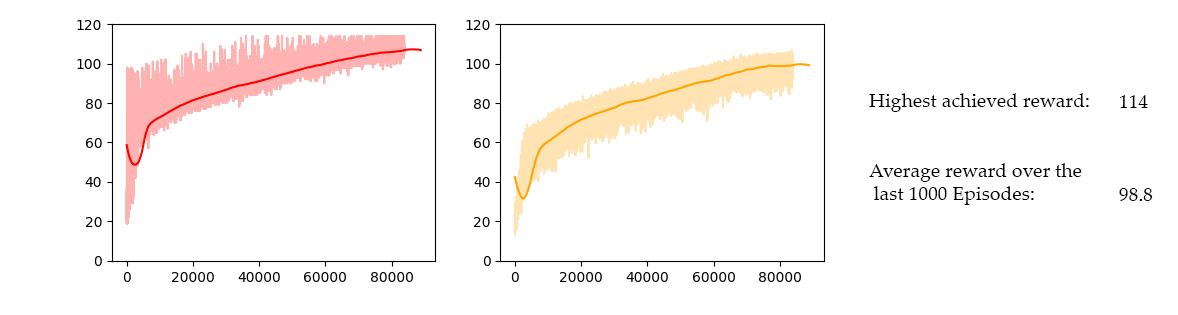
\includegraphics[width=1\textwidth]{Figures/plots/plot_gz_acktr.png}
  \caption{Reward per Episode for the Gateway vs Zerg Scenario with maximum over all environments(left) and mean over all environments(right)}
  \label{fig:gz_rew}
\end{figure}

As Figure \ref{fig:gz_rew} shows, the network actually got worse than random actions for the first few thousand episodes, followed by a short but steep ascend, after which it then slowly and steadily improved until training was stopped after approximately 83000 Episodes per Environment. For this scenario there is largely no difference between mean and max plots as the results were very consistent across environments and on an episode to episode basis.

All of the aforementioned human strategies were learned almost perfectly by the algorithm. It cuts the enemy army in half, and not just randomly, but purposefully in a way that most if not all enemy melee units are on one side and all ranged units on the other for maximum effectiveness. It also conserves energy by placing the forcefields considerably more efficient than was observed in the human tests. Where humans most of the time used 7-8 forcefields very quickly, the algorithm on average only needs 4-5 forcefields to cut the enemy army in half. After that it simply waits and uses the saved energy only if one of the forcefields expires in order to shore up the hole that was left by it or if the enemy units manage to actually get around the existing forcefields. 

\begin{figure}[htb]
  \centering
      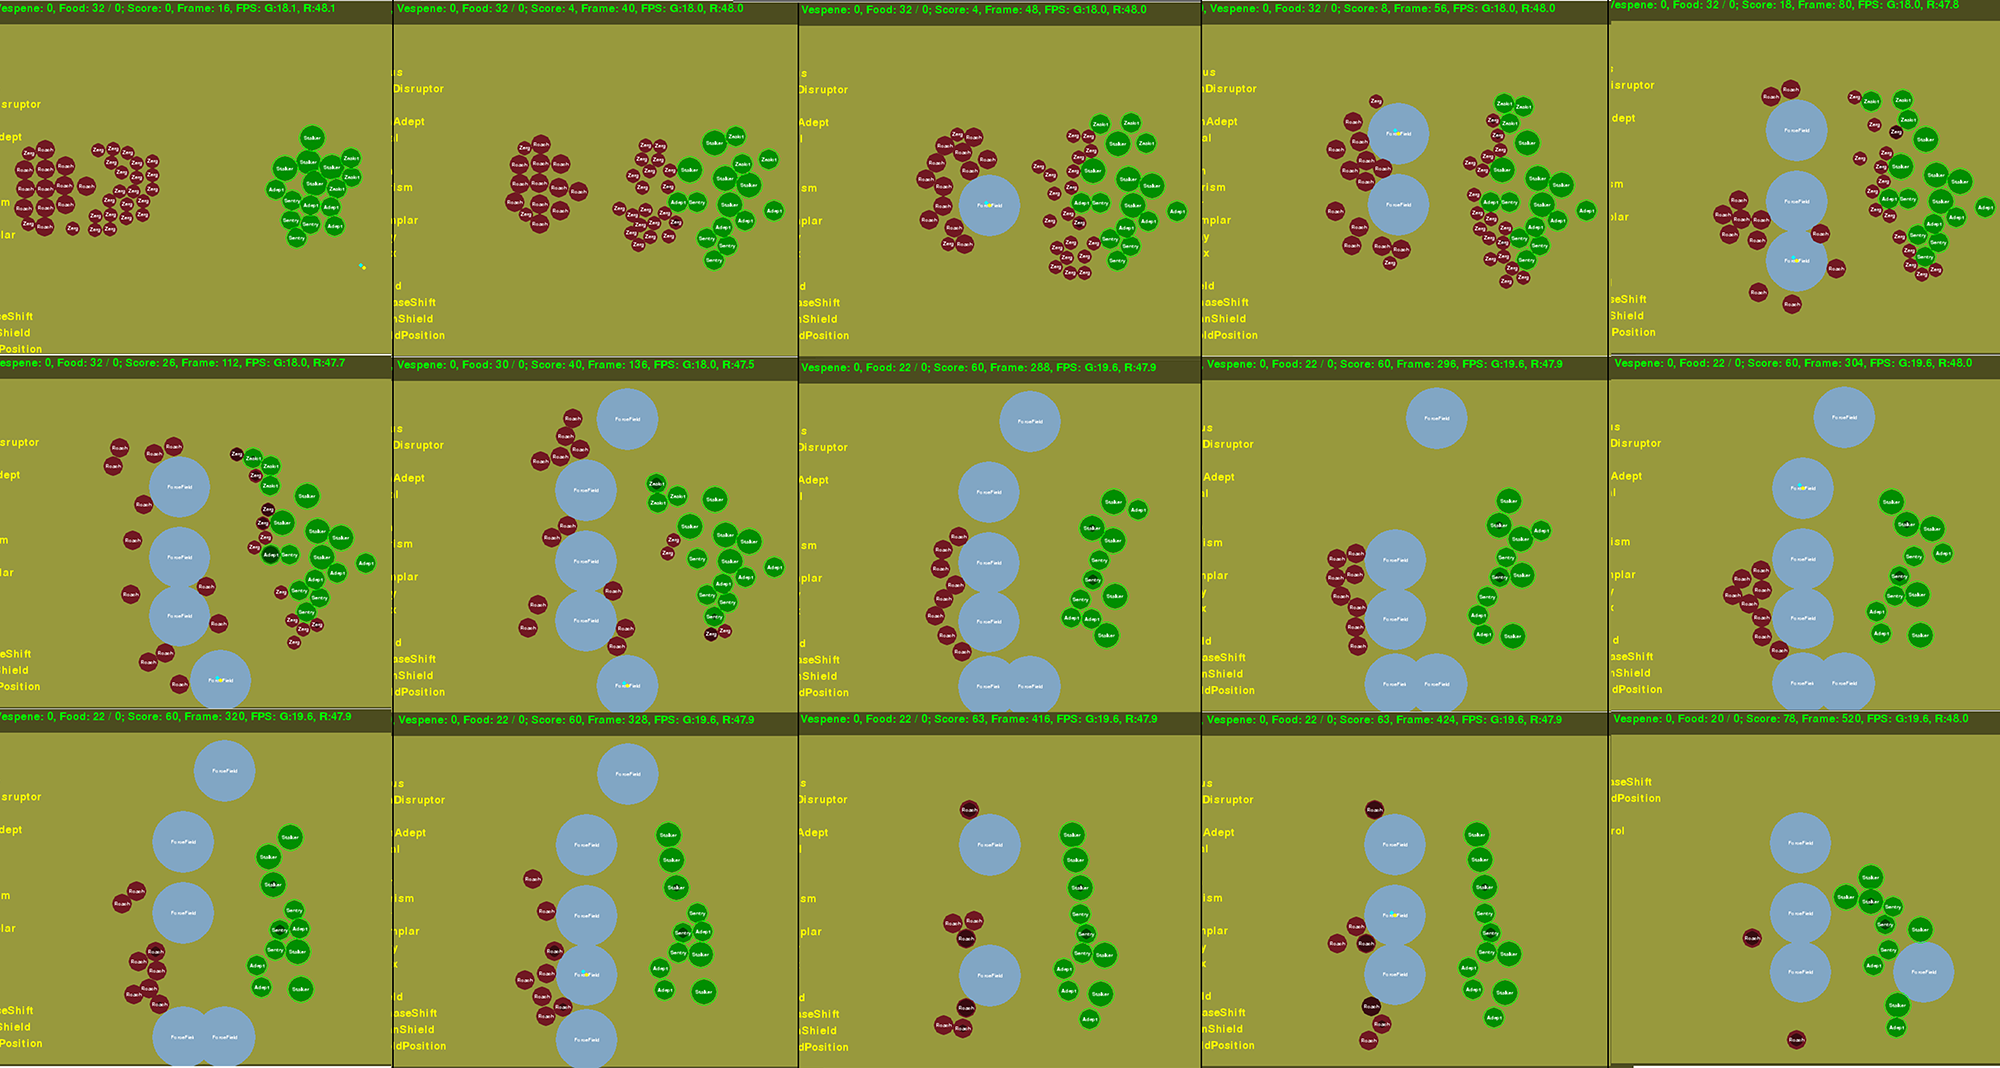
\includegraphics[width=1\textwidth]{Figures/gz_strategy.png}
  \caption{ A Sequence of select state snapshots using a trained model on the Gateway vs Zerg Scenario. The network places the forcefields(blue) strategically to disrupt the enemy army and keep ranged units from attacking the own army}
  \label{fig:gzstrat}
\end{figure}

Figure \ref{fig:gzstrat} illustrates this exact behaviour, showing one episode in which almost maximum rewards were achieved. The only misstep that was made in this episode is right at the end, where a forcefield is placed inside of the players army, but there are not enough enemy units left over to capitalize on this mistake, which is likely why the network has not unlearned or discouraged this behaviour.
\subsection{Scenario Comparison}

\begin{table}[htb]
\centering
\begin{tabular}{@{}llllll@{}}
\toprule
Scenario                 & $s_1$ & \begin{tabular}[c]{@{}l@{}} $s_2$\end{tabular} & \begin{tabular}[c]{@{}l@{}} $p_1$\end{tabular} & \begin{tabular}[c]{@{}l@{}} $p_2$\end{tabular} & \begin{tabular}[c]{@{}l@{}}$p_3$\end{tabular} \\ \midrule
FindUltralisk            & 46                 & 31.0                                                                                                         & $\sim$92\%                                                                                    & 68\%                                                                                         & 64\%                                                                                            \\
FindUltraliskWithCreep   & 46                 & 23.2                                                                                                         & $\sim$100\%                                                                                   & 62\%                                                                                         & 54\%                                                                                            \\
GatewayZerg              & 114                & 98.8                                                                                                         & 92.3\%                                                                                        & 156\%                                                                                        & 99\%                                                                                            \\
StalkerRoaches           & 100                & 43.3                                                                                                         & 100\%                                                                                         & 72\%                                                                                         & 45\%                                                                                            \\
ReaperZergling(Cheating) & 19                 & 7.6                                                                                                          & 100\%                                                                                         & 44\%                                                                                         & 40\%                                                                                            \\
ReaperZergling           & 19                 & 5.4                                                                                                          & 100\%                                                                                         & 31\%                                                                                         & 28\%                                                                                            \\ \bottomrule
\end{tabular}
\captionsetup{singlelinecheck=off}
\caption[]{Summary of Scenario evaluations. \\ Column Definitions:
\begin{itemize}
\item $s_1$ - Maximum Score obtained
\item $s_2$ - Average Score obtained over last 1000 Episodes across all Environments
\item $p_1$ - Percentage for $s_1$ of maximum Score possible
\item $p_2$ - Percentage for $s_2$ of novice Player baseline
\item $p_3$ - Percentage for $s_2$ of advanced Player baseline 
\end{itemize}
}
\label{tab:scen_eval}
\end{table}

Table \ref{tab:scen_eval} compares the best results that were able to be obtained in each scenario. Both the maximum scores ($s_1$, $p_1$) and an average over 1000 Episodes after a policy was learned ($s_2$) are compared and put into the context of human player's results ($p_2$, $p_3$). The percentages calculated for the maximum reward $p_1$ are adjusted for the minimum possible reward as well, where it differs from 0. This makes an especially big difference in the GatewayZerg scenario, where the minimum reward is already ca. 45.  

Some of these results conform roughly with the expectations that were held at the beginning of this thesis. The Find Ultralisk and Find Ultralisk with Creep scenarios were solved with considerable success, albeit not quite as consistently as either of the human players. The Stalker vs Roaches scenario, as expected, posed much more of a challenge and the algorithm was not able to learn the "correct" strategy, which shows in the average rewards it obtained. Nonetheless, even it's suboptimal policy managed to achieve maximum rewards at least sometimes.

There were also big surprises however. The algorithm performed much better than expected in the Gateway vs Zerg scenario. It being the most difficult scenario for humans the algorithm was expected to have quite a few problems with it as well, but it managed to become just as good as the advanced human player. It is particularly surprising how consistently high scores were achieved in comparison with all other scenarios, where even after learning the optimal strategy the obtained rewards span the entire range of possible rewards in the environment. The reason this scenario might be easier for reinforcement learning algorithms than the other scenarios is that it exhibits slightly less randomness for a computer at least. A large part of the randomness and difficulty felt by humans in this scenario comes from not being able to predict the movement of enemy units around the forcefields during split second decision making. This pathing is actually deterministic however. Therefore if an algorithm is able to predict this movement, this scenario becomes much easier, as there are fewer differences between states of different episodes, if similar movement patterns can be forced by similar forcefield placement.

A surprise in the opposite direction were the results of the ReaperZergling scenario. Initially thought to be the easiest of the three competitive scenarios it turned out to be the scenario the algorithms had the most difficulty with. As can shown by the results in table \ref{tab:scen_eval} even with cheating the algorithm only managed to obtain 44\%/40\% of the human players' scores. This is due to the fact that, while sitting in the corner where the units cannot be reached easily guarantees a high score, getting to that spot is still somewhat difficult and could not be done consistently. This is likely owed to the enemies' very fast movement being hard to predict because of the unorthodox terrain and pathing mechanisms. Without the possibility of simply hiding the algorithm faired even worse, achieving only 31\%/28\% of human scores. In both versions the algorithm was able to achieve the maximum score of 19 every once in a while though.

In conclusion the FindUltralisk and FindUltraliskWithCreep scenarios do the job of introductory scenarios quite well, but the GatewayvsZerg scenario works just as well if not better, while also being a scenario that reflects the actual game. These results also show, that scenarios that are somewhat difficult for human players can be very easy for reinforcement learning algorithms and vice versa.

\section{Algorithms}
\label{sec:eval_algo}

This section will compare the three algorithms that were used in this project in their usefulness for StarCraft II Reinforcement Leaning. This section however was hit hardest by the resource and time constraints, as after trying to solve all scenarios using the ACKTR algorithm there was not enough time to tune both other algorithms adequately for all of them. This means that some scenarios, especially the more difficult ones, were left entirely unsolved by the A2C and A3C algorithms.

From OpenAI's blog post \citep{openaiblog-a2c} and other sources the initial expectation was that ACKTR will outperform A2C and A3C by a considerable margin. In the few comparisons that can be made, this expectation was not only confirmed, but the differences seem to be even greater than anticipated. The easiest scenario, Find Ultralisk, is the only scenario where all three algorithms were able to obtain close to optimal results with any kind of consistency. Nonetheless, it already highlights one of the big problems with the A3C implementation. After the A3c algorithm was able to learn a policy that achieves decent rewards it, sometimes almost instantly, unlearns this policy a few hundred or thousand episodes later as seen in Figure \ref{fig:a3c_unlearn}. This happens even with relatively small learning rates, that should only allow small adjustments to be made to the network weights, which might indicate a bug in the implementation, but that could not yet be determined.    
\begin{figure}[htb]
  \centering
      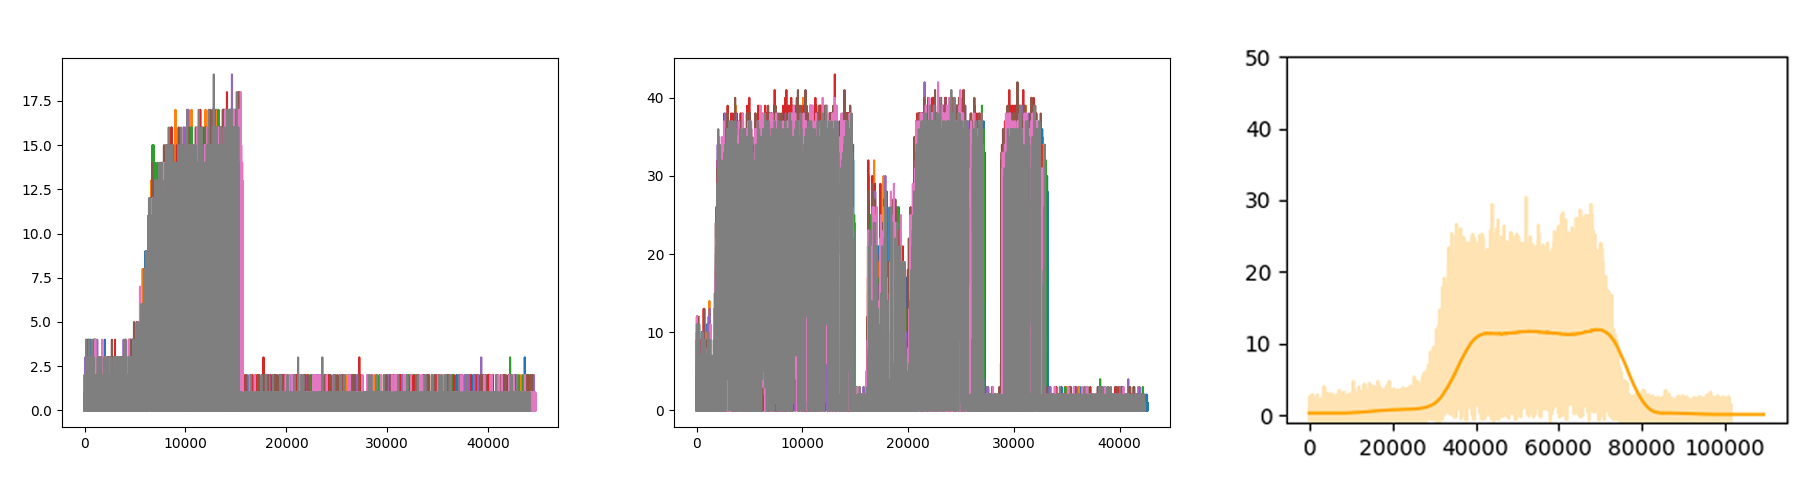
\includegraphics[width=1\textwidth]{Figures/plots/a3c_unlearning.png}
  \caption{Different examples of the problem of policy fragility in the A3C Algorithm. Scenarios from left to right: FindUltralisk(simplified), FindUltraliskWithCreep(simplified), FindUltraliskWithCreep(proper). The rightmost plot also shows how much worse the A3C performed in general, with an average score of only 12 points during it's peak in  the FindUltralisk Scenario}
  \label{fig:a3c_unlearn}
\end{figure}

The GatewayZerg scenario, although quite easy for the acktr algorithm, could not be adequately learned by the A3C algorithm, as shown by Figure \ref{fig:gz_a3c}. The policy learned is only a very slight improvement over the random policy and is not comparable with the human players.

\begin{figure}[htb]
  \centering
      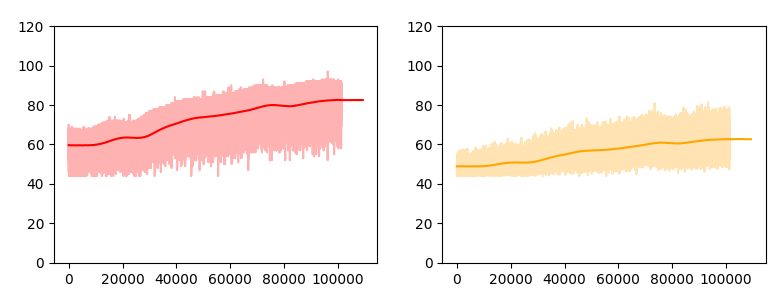
\includegraphics[width=0.8\textwidth]{Figures/plots/gz_a3c.png}
  \caption{Performance of the A3C algorithm in the GatewayZerg scenario. While small improvements were made, the policy obtains still largely random scores.}
  \label{fig:gz_a3c}
\end{figure}

For the ReaperZergling and StalkerRoaches scenarios no meaningful policy could be learned at all by the A3C algorithm.

The A2C algorithm did not exhibit the unlearning problem of the A3C algorithm and for the FindUltralisk scenario in it's simplified variant was even able to beat the ACKTR algorithm with the scores depicted in Figure \ref{fig:a2c_fu}. This is the only scenario that the A2C algorithm successfully learned however, and the fact that it beat the ACKTR algorithm is likely due to differently tuned hyperparameters and not an indicator that the A2C algorithm is superior.

\begin{figure}[htb]
  \centering
      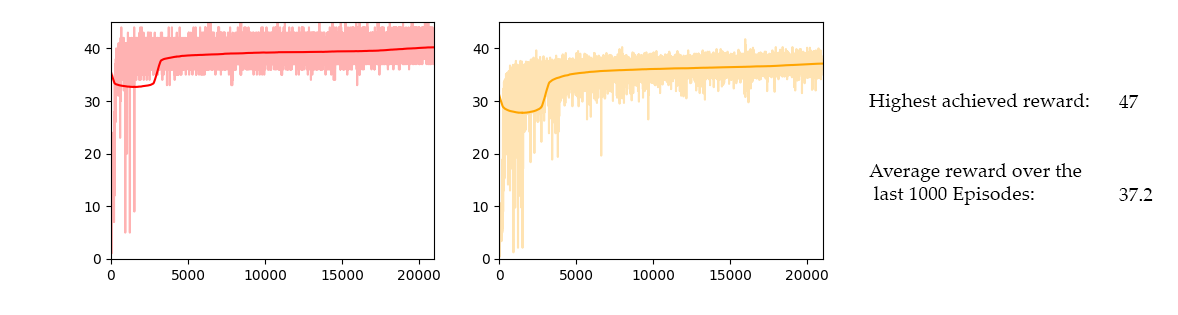
\includegraphics[width=1\textwidth]{Figures/plots/a2c_fu.png}
  \caption{Performance of the A2C algorithm in the FindUltralisk scenario in it's simplified variant. The peak average reward of 37.2 beats even the ACKTR algorithm that only managed 32(cf. Figure \ref{fig:simplevs_fu}). }
  \label{fig:a2c_fu}
\end{figure}

Nonetheless, even the FindUltraliskWithCreep scenario posed very big problems for the A2C algorithm, where it only managed to learn not to step on creep surfaces therefore obtaining exactly 0 reward points in each episode. This was the case in both the simplified variant and using screen coordinates. For this reason no other scenarios were attempted with this algorithm.

One big advantage of the ACKTR algorithm seems to be that it is much less dependent on very precise hyperparamater tuning than A2C and A3C as far as the learning rate is considered. As illustrated in section \ref{sec:lr} atleast for the FindUltraliskWithCreep scenario, there exists a wide range of learning rates that result in decent performance, whereas with the A3C algorithm for example adjustments with precision of $10^{-5}$ were needed to exhibit any information gain at all. 

\section{Simple vs action arguments}
\label{sec:eval_aa}
The next comparison to be done is between the different action representations for the policy, specifically between the simplified versions and the versions featuring screen coordinates.
This comparison can not fully be done over all scenarios, and for this reason this section will only feature scenarios that have a simplified variant. 

Originally a third strategy was meant to be added to this comparison, the flattening approach, which simply merges arguments and actions into a one dimensional array. This would have been a good measure for determining how beneficial it is to separate action and screen coordinate outputs from the neural network, but this part of the comparison could not be completed in time for this thesis.

In general it can be said, that the simplified variants were learned faster and more smoothly than the variants making use of actual coordinates. The simplification is not without drawbacks however, as in the end most models using action arguments were able to obtain at least slightly higher rewards more consistently than the models trained with the simplified actions. This is largely owed to the fact that  units can simply be moved more efficiently with precise coordinates in comparison to the grid like movement they are constrained to by the abstract actions. Figure \ref{fig:simplevs_fu} shows these differences in the FindUltralisk scenario.

\begin{figure}[htb]
  \centering
      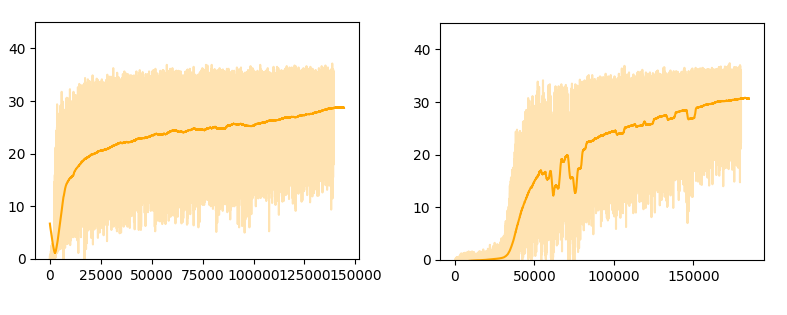
\includegraphics[width=0.8\textwidth]{Figures/plots/acktr_fu_simplevs.png}
  \caption{Comparison of simplified version(left) and version with action arguments(right) in the FindUltralisk scenario.}
  \label{fig:simplevs_fu}
\end{figure}

The results for the FindUltraliskWithCreep scenario depicted in Figure \ref{fig:simplevs_fuwc} are similar. The test run for the simplified version sadly had to be terminated prematurely, but the rewards seemed to mostly stagnate so this comparison still holds. The simplified variant again was learned much faster but with less maximum and average rewards in the long run.
\begin{figure}[htb]
  \centering
      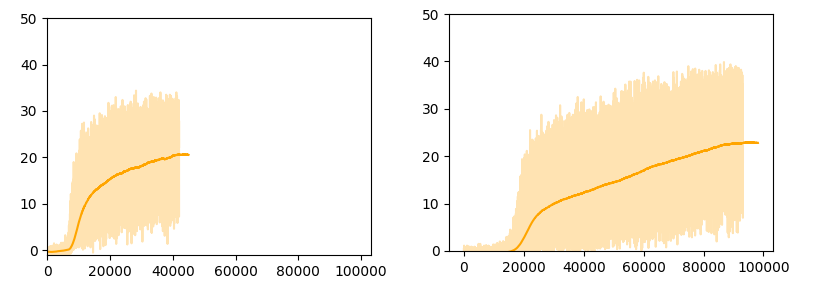
\includegraphics[width=0.8\textwidth]{Figures/plots/fuwc_simplevs.png}
  \caption{Comparison of a short run of simplified version(left) and version with action arguments(right)in the FindUltraliskWith scenario.}
  \label{fig:simplevs_fuwc}
\end{figure}

The Reaper vs Zergling Scenario exposes an even larger problem with the abstracted actions of the simplified versions. Due to the way StarCraft II's internal pathfinding algorithm determines the actual path that the units take in order to get to the coordinate specified by the player during any action that requires movement, the grid-like movement can lead to very unintuitive results, when there are obstacles or terrain changes in the path of the unit. This is because the pathfinding algorithm will automatically choose an optimal path around all obstacles and also up or down different terrain height levels.

An additional problem for the simplified actions that arises in any scenario involving different terrain heights is the fixed distance, that the unit is ordered to move in each step, which increases the discrepancy even further between where the unit is ordered to move to and where the pathfinding algorithm actually moves it towards in the next step.


\section{Impact of Sample Diversity by Environment Parallelisation}
While not strictly related to the StarCraft II environment, for the purpose of performance testing it was determined how much the diversity of samples gained by using a number of parallel environments improves sample efficiency. This was considered important, as training slows down with too many environments meaning this sample efficiency has to be weighed against time efficiency. Tests were done on the somewhat easy Find Ultralisk With Creep Scenario to ensure that even if missing sample diversity is a large problem for the ACKTR algorithm, it should still able learn at least something. The number of parallel environments tested are 1, 2, 8, 16 and 32.

For this evaluation the plots were generated slightly differently than before. In order to better compare the results no average was made across the environments, and instead the results of each environment are merged into one plot in a zipper like manner. Looking at the graphs one can still see a large difference in the number of episodes, that were run in each test, but this can be attributed to the varying length of episodes, all tests were run for exactly 80 million time steps.

\begin{figure}[htb]
  \centering
      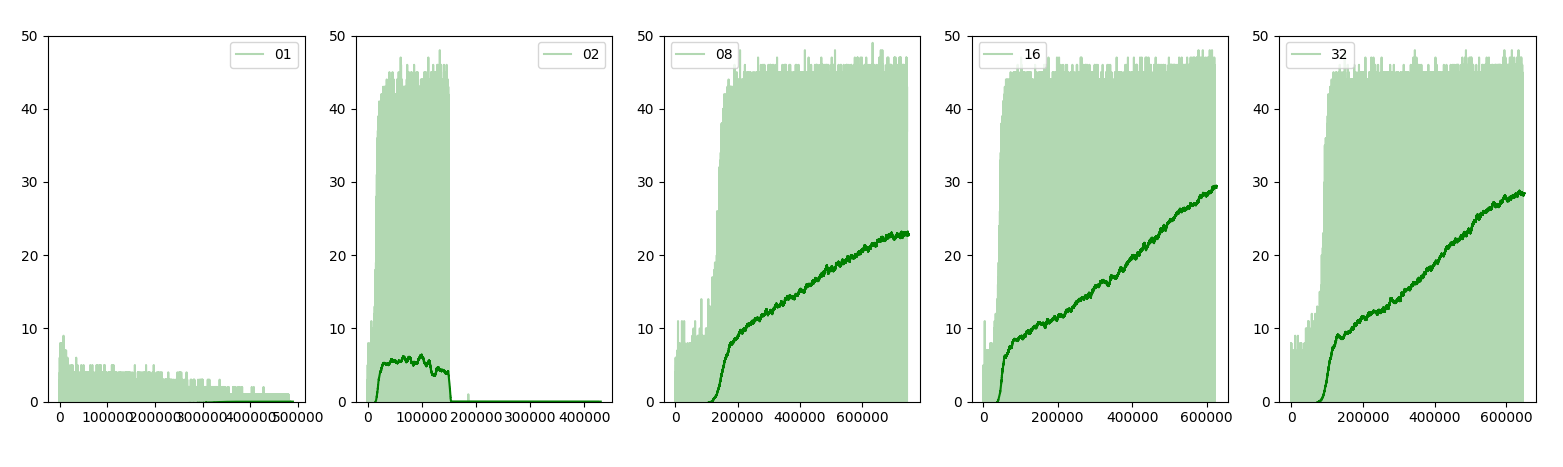
\includegraphics[width=1\textwidth]{Figures/plots/acktr_diversity.png}
  \caption{Effect of the number of parallel environments on the training process of the ACKTR algorithm. Tested on the Find Ultralisk With Creep Scenario using Action Coordinates. x-Axis: Episode number, y-Axis: End of Episode Reward}
  \label{fig:acktr_diverse}
\end{figure}

Figure \ref{fig:acktr_diverse} shows the result of these tests. These graphs make quite clear, that sample diversity is in fact very important for the ACKTR algorithm. Using only very few  parallel environments might even prevent learning entirely, as shown by the test run with only 1 environment. With 2 environments there was some success at first, almost mirroring the initial reward ascend of the other test runs, but then quickly plateaued and even unlearned everything after a short time, showing that it is much less robust. \\ The difference between the other 3 test runs is much smaller, but still considerable. Utilizing 16 or 32 parallel environments enabled the algorithm not only to learn faster, but also reach higher overall rewards and consistency in comparison with 8 environments, which were used for almost all tests over the course of this thesis. These results indicate, that choosing the number of environments is not only a question of sample efficiency vs time efficiency, but that it might be necessary to utilize a very high amount of parallel environments, to learn an optimal policy.


\section{Impact of different learning rates}
\label{sec:lr}
As the learning rate was the main hyperparameter that was tuned over the course of this project this section contains an analysis how different learning rates affected training in these environments. Tested was only the ACKTR algorithm and tests were made starting with a learning rate of 0.5 which was progressively divided by 10 for each further test. All tests were made on the relatively easy Find Ultralisk With Creep Scenario to ensure, that most of these learning rates get a result, and all tests ran for 80 million steps. Using a relatively easy scenario also shows that using too small of a learning rate can also result in no knowledge gain at all. Figure \ref{fig:acktr_lr} demonstrates this. 

\begin{figure}[htb]
  \centering
      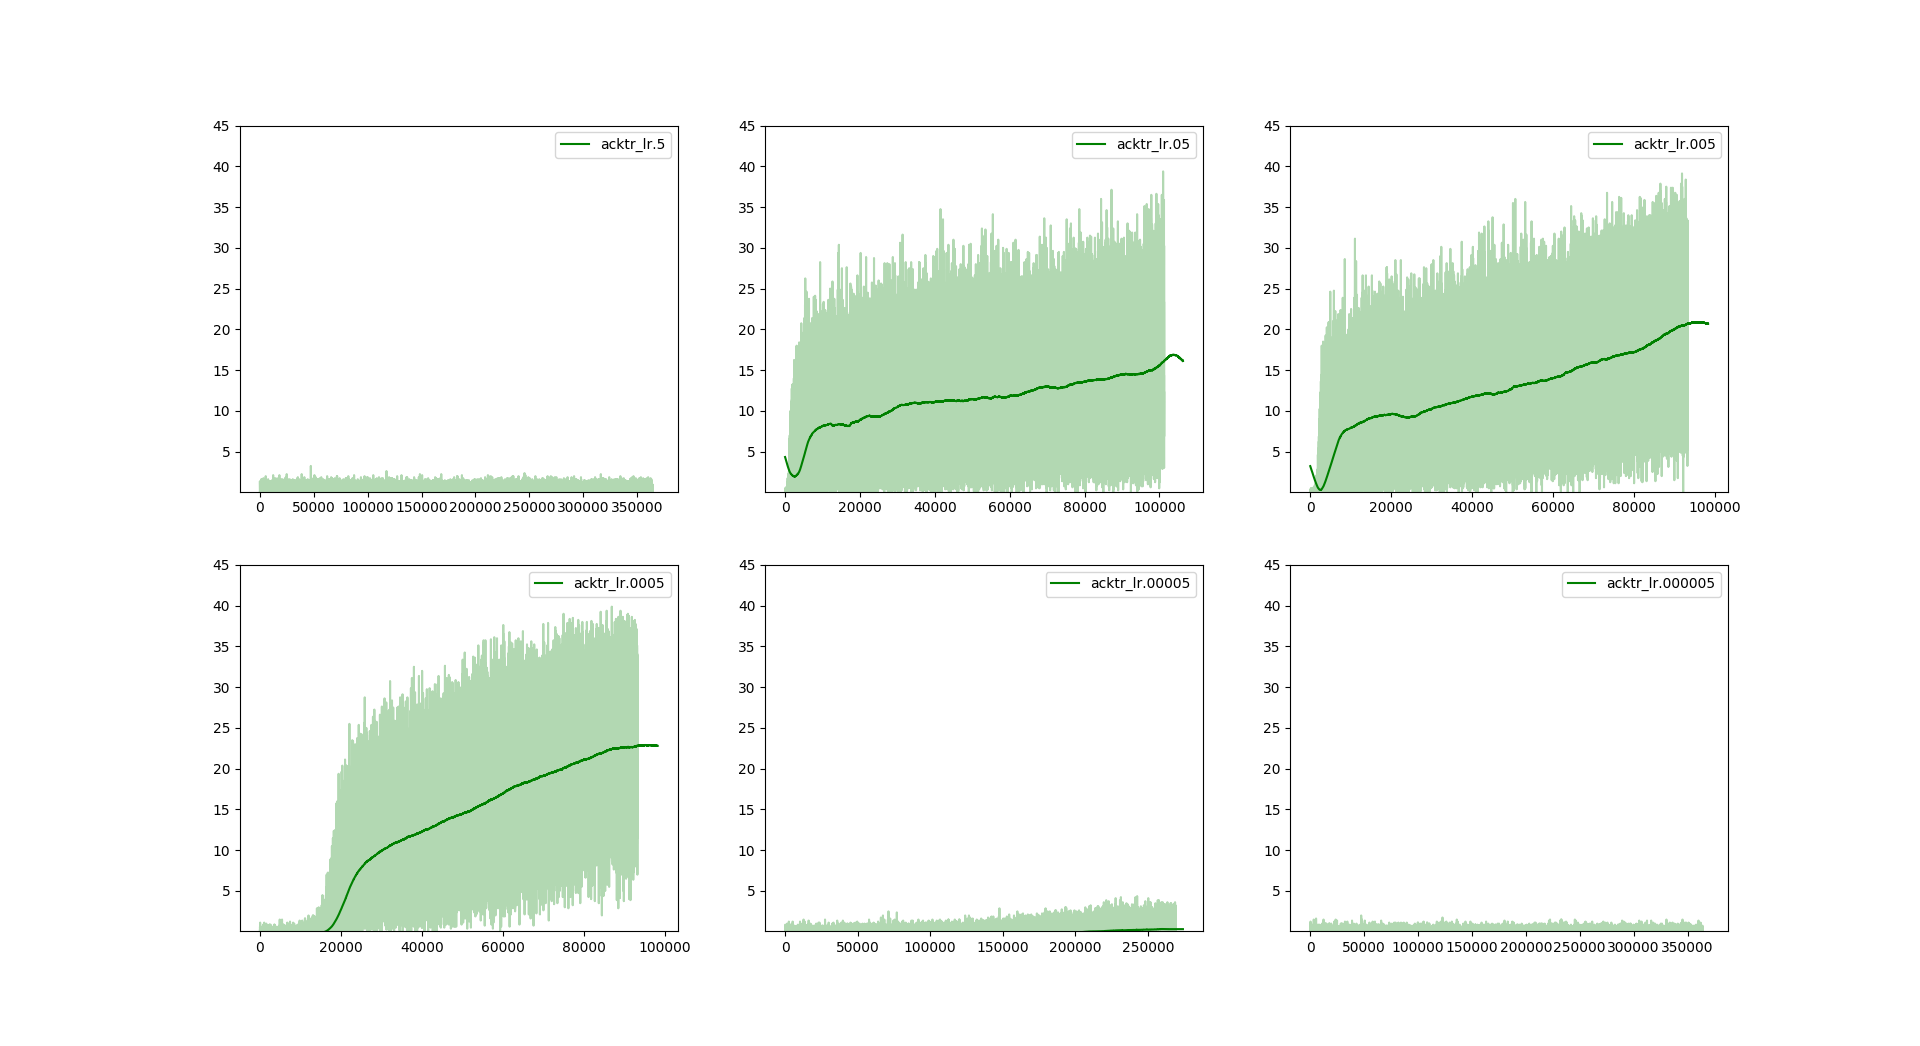
\includegraphics[width=1\textwidth]{Figures/plots/acktr_lr.png}
  \caption{Effect of different learning rates on the training process of the ACKTR algorithm. Tested on the Find Ultralisk With Creep Scenario using Action Coordinates. x-Axis: Episode number, y-Axis: End of Episode Reward}
  \label{fig:acktr_lr}
\end{figure}

In this specific scenario only learning rates between 0.05 and 0.0005 result in any training at all. The best result was achieved using the 0.0005 learning rate, where the reward ascend is very smooth and the highest overall rewards were experienced. Nonetheless the rewards were gained much later than when utilizing higher learning rates,  as for the first about 18000 episodes per environment no rewards were achieved at all, whereas higher learning rates achieved noticeable rewards almost immediately.Their reward ascend is more erratic and slowed down considerably after an initial period of very steep gains however.

In concurrence with these findings the goal for learning the other scenarios optimally was to find he lowest possible learning rate, that still results in learning in a reasonable amount of steps.  


\section{Impact of a state history}
This section compares 2 test runs on the Find Ultralisk with Creep Scenario. One with only a single timestep functioning as the state of the environment, and the other utilizing a history of 4 states.

\begin{figure}[htb]
  \centering
      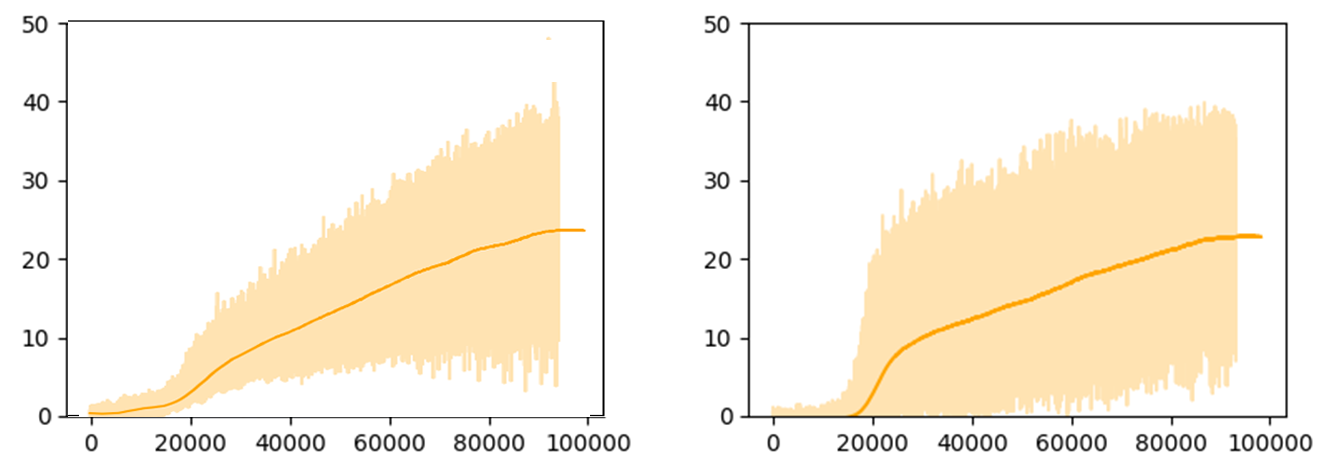
\includegraphics[width=1\textwidth]{Figures/plots/fuwc_history.png}
  \caption{Comparison between utilizing a history of 4 timesteps(left) as observations with a single timestep state(right). Tested on the Find Ultralisk With Creep Scenario using Action Coordinates. x-Axis: Episode number, y-Axis: End of Episode Reward}
  \label{fig:acktr_history}
\end{figure}

As Figure \ref{fig:acktr_history} shows, the end results of both test runs are not substantially different, although the end rewards were slightly higher while using a state history. The largest difference is, that the training curve was smoothed out a considerable amount and results have become somewhat more consistent. This improvement in consistency became much smaller towards the end of the training run however, and in the end they are both almost equally inconsistent. 

As the player in the FindUltraliskwithCreep Scenario does not especially benefit from knowing the last few states, which is also the case for all other scenarios in this thesis, this rather small difference between state history and no state history was more or less expected. 
Because training with the state history took more than twice as long one can conclude, that if the specific scenario to be trained does not necessitate the usage of a state history, or there is some obvious information gain one should likely elect not to use such a state history.  


\section{Impact of Learning from Replays}
The attempt to incorporate human replay experiences into the training process did not go as well as had been initially hoped. 
Both the strategy to slowly add replay samples over time, and the strategy to dump all human experiences before the actual reinforcement learning process begins did not manage to improve the performance or conversion properties of the A3c algorithm in the FindUltraliskWithCreep Scenario.

While the "kick-start" strategy had almost no effect in all cases even when feeding the experiences into the network multiple times, the other strategy did even worse by lowering performance or even preventing training entirely for any but very slow percentages of human replays added. Figure  \ref{fig:a3c_replay} shows a comparison between regular training and the "kick-start" strategy. The largest difference is, that using the human replay experiences the algorithm managed to retain a proper policy for a slightly longer time than without, before unlearning it. This effect however, is largely random and can also be found between multiple runs without replay experiences and can therefore not be seen as an improvement. 

\begin{figure}[htb]
  \centering
      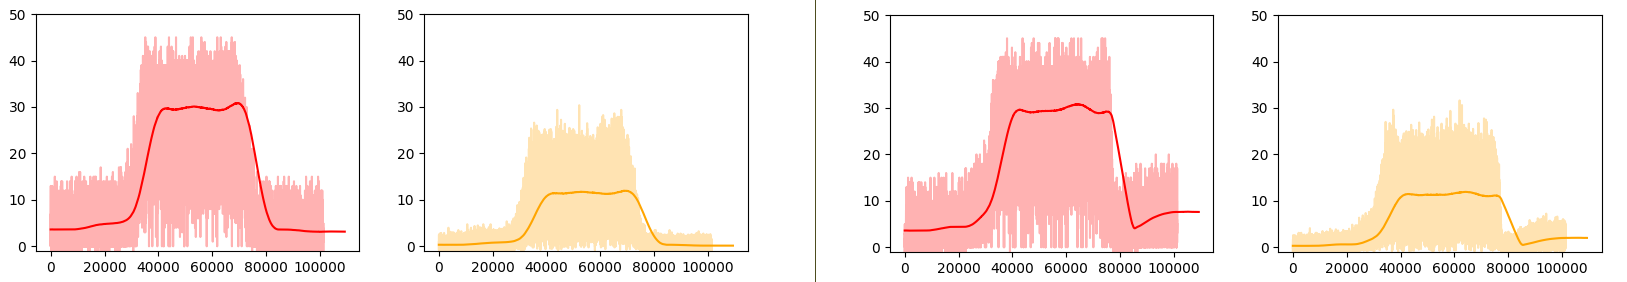
\includegraphics[width=1\textwidth]{Figures/plots/a3c_fuwc_replays.png}
  \caption{Comparison between a test run with added human replay experiences(right) and a standard test run(left) on the Find Ultralisk With Creep Scenario utilizing the A3C algorithm}
  \label{fig:a3c_replay}
\end{figure}

The second scenario that this was attempted on was the ReaperZergling scenario, where the A3c algorithm was not able to learn any meaningful policy without the human experiences and it was hoped, they could change that. Nonetheless, no improvements could be made in this scenario either.

There are multiple reasons that could have led to the failure of this attempt. The largest problem is likely the comparatively insignificant amount of human data of only 1400 steps that was recorded for these tests compared to the 80 million steps done during normal training. For the Find Ultralisk With Creep Scenario they make up only around 30 episodes. In contrast, the a3c algorithm needed around 1000 times more episodes to learn a meaningful policy during regular training. It is therefore easy to see, why they would only have little recognizable impact.

The strategy of slowly adding samples over time adds many more human samples to the network by duplication, which alleviates the previous problem, but introduces a new one. Having tens of thousands or even hundreds of thousands of samples out of the same small set of samples likely introduces overfitting to these exact state spaces. This might also hinder exploration by making the policy more deterministic, counteracting the entropy.

The "kick-start" strategy has one additional drawback, due to the importance of the current value function estimate for calculating the discounted rewards. As all samples are added before the actual training, the value function estimate of the neural network is still largely random or a very rough estimate at best as more of the samples are added. This can not give an accurate representation of the discounted reward.




